% Chapter 3

\chapter{System Design} % Chapter title

% For referencing the chapter elsewhere, use \autoref{ch:design}
\label{ch:design}

%TC:ignore
%This is the System Design chapter, should be approximately 4,000 Words in total.
%The PUF section should be approximately 1,250 words long.
%The main Fuzzy Extractor section should be approximately 1,250 words long
%Cryptographic Hashing section, it should 750 words long.
%Networking section should be 750 words in length.
%TC:endignore
%-------------------------------------------------------------------------------


\section{Introduction}

Ideally, a complete \gls{puf}-based authenticatable device could be implemented
on a single \gls{fpga}, containing all the necessary components required.
However, given the time constraints of a Masters project, while this approach
was initially favoured, it was deemed necessary to simulate parts of the system
in the \matlab programming environment. The system area considered most
difficult to synthesise was the error correction encoder and decoder.
These are critical components, without which a Fuzzy Extractor could not be implemented.
As a result, both the generator and reproduction implementations of the Fuzzy Extractor
were not implemented in \gls{fpga} but simulated.

The Ethernet protocol is also comparatively complex and so modification of this
for the purposes of device authentication was also removed from the design.
Instead, a study of possible protocol schemes was conducted with
a simulation of only one message of the complete scheme developed to a level
for demonstration.

The \gls{puf} functionality of \gls{sram} on the other hand,
 was possible for full implementation in \gls{fpga}, due to the easy
availability of multiple DE-1 development boards, each with integrated \gls{sram} chips.
Extraction of specific \gls{puf} data from the \gls{sram} chip would require the design of
a `wrapper' function that could issue memory addresses and retrieve memory
contents of the \gls{sram} chip. It would then be necessary to link that wrapper
with a communication system that would allow external access to the device.

It was decided to implement this system using the RS-232 protocol standard.
This is because the necessary hardware was available on the DE-1 board and it was
deemed the simplest to implement.
The development of a UART that could receive memory address locations encoded
serially and pass them in full to the wrapper was thus required.
Likewise, it would be necessary to send the memory contents passed from the
wrapper serially back to the requester.
This requester would be a full PC running \matlab which contains
the ability to integrate serial communications data into its programs.

\section{SRAM-PUF interface implementation on FPGA}

The SRAM-PUF interface was designed in three sections each in a seperate \gls{vhdl} file.
These files can be found in the appendix and can be summarized as follows:
\begin{description}
\item[SRAM.VHD] \hfill \\
  Used as a `wrapper'. Required to access the \gls{sram} memory.
\item[UART.VHD] \hfill \\
  Used to interface between the SRAM wrapper and the physical RS-232 connection.
\item[PUF.VHD] \hfill \\
  Used to connect the above two sections together and connect their inputs and outputs
  to the appropriate pins of the FPGA to communication with the peripherals which included
  the SRAM chip, the MAX232 RS-232 driver/receiver chip, master clock, reset button and
  LED array.
\end{description}

\subsection{SRAM wrapper}

The DE-1 development board contains a IS61LV25616 chip. This contains
$2^{22}$ SRAM cells organised into $2^{18}$ words of 16-bits each. A memory of this size
provides more than sufficient quantity of memory for testing our design.
In fact, for the purposes of simplicity, it is easier to use only a quarter
of the address space the chip provides, to allow 16-bit addressing which
reduces the complexity of the communications (via RS-232) part.
The implementation of the \gls{sram} `wrapper', as it came to be known, involved coding a
component in VHDL to be synthesised for use on the \gls{fpga} of the DE-1 development board
This can be split into two areas of responsibility; a \emph{transmit} and a \emph{receive}
section. Both were implemented in a single \gls{vhdl} process sensitive to the master
clock to make \gls{rtl} synthesis less complex to design for and debug.

The receive section was required to convert multiple 8-byte words received from the
\gls{uart} module into one 16-byte memory address word to be placed on the memory bus
connected to the \gls{sram} chip. The transmit section was required to perform the opposite function of
converting a single 16-byte data word output into multiple 8-byte words.

To access the \gls{sram} chip as a \gls{puf}, we need only to concern ourselves with
the read cycle of the device, as writing data is counter-productive.
There are 5 control lines to the chip (all
use active-low);
Chip Enable ($\overline{CE}$),
Write Enable ($\overline{WE}$),
Output Enable ($\overline{OE}$),
Lower Byte Access ($\overline{LB}$) and
Upper Byte Access ($\overline{UB}$).

Whilst the first three can remain in a constant state for our purposes
($\overline{CE} = 0, \overline{WE} = 1, \overline{OE} = 0$), the byte access signals
can be utilized to output the full 16-bit memory data onto just one 8-bit bus
by cross-wiring the low order bits lines (0-7) to the high order bits (8-15)
sequentially.
Therefore, a full reading can, in theory, be sent via the rs-232 link in two transmissions.
In a similar way, the 16-bit address can be received in two pieces.
Timing is important, and the particular chip on the development board is the
fastest in the range, with an access time of 10ns rather than 12ns or 15ns in
other chips in the family.
Thus, with careful reading of the datasheets\cite{sramdatasheet}, from
the initial setting of the address to the point at which the data output is
valid\footnote{$t_{AA}$, or Address Access Time} is 10ns.

It can be seen that a wrapper function is required that buffers the two part address
as it is received, then \emph{forwards} a complete 16-bit address onwards to
the address bus of the \gls{sram} memory, with the \gls{uba} signal active.
After some delay greater than 10ns, the upper byte can be forwarded and the
upper and \gls{lba} signals toggled. After at least another identical delay,
and if a strobe has been received from the communication module to indicate the previous
byte has been sent, the lower byte can be forwarded. This creates a system for
converting challenges in the form of memory addresses into responses in the form of
memory data.

This was indeed the first configuration of the wrapper function implemented, however over time
it became apparent that due to the encoding of some memory addresses as ASCII escape
characters used in RS-232, certain memory locations were effectively unavailable.
Specifying them in a challenge would cause unspecified behavior (bugs). Thus, a more redundant
encoding scheme for the addresses needed to be used.

It would be preferable to implement the system such that all memory
addresses could be specified without accidentally encoding a `system bell',
`carriage return' or, most dangerously, the RS-232 software flow control sequences
`XOFF' and `XON' which could end the communication session abruptly.
For this purpose, the wrapper was extended to separate a 16-bit memory address into four
4-bit values (nibbles) each rather than just two 8-bit values. A simple scheme was used
whereby these 4-bit values could be encoded as an \gls{ascii} character corresponding to their
value in conventional hexadecimal notation. This turned out to be very useful in testing
as faults could be detected in short order if non-hexadecimal characters appeared in
any terminal output from the device. Note that \gls{ascii} is a 7-bit encoding, but for
the purposes of this project it is considered as 8-bits where the \gls{msb} is always `0'.

In encoding 4-bits of binary data to and from \gls{ascii} a conditional statement,
two possibilities could be used:
\begin{description}
\item[Numbers] \hfill \\
  The binary 4-bit values `0000' to `1001' (0-9) could be encoded as \gls{ascii} numerical
  characters. This means that the upper nibble must be set to `0011' and the lower bit is
  the binary value (a useful property of \gls{ascii})
\item[Letters] \hfill \\
  Binary values greater than `1001' (decimal 9) need to be represented as the \gls{ascii}
  characters A-F which in binary are represented in the 8-bit values; `01000001' (decimal 65) to
  `01000110' (decimal 70). So, for conversion, the upper nibble must be set to `0100' and
  the lower nibble is the binary value plus the value `1001' (decimal 9).
\end{description}

Similarly, converting an \gls{ascii} byte to a binary nibble requires another conditional
statement in VHDL. This time it is slightly more complicated, as one more condition is
added to accommodate for lowercase characters (a-f) in the input,
where the upper nibble is `0110' instead of `0100'.

This final implementation abandoned the use of the \gls{uba} and \gls{lba} toggling and
instead used a loop structure to access each nibble of the full 16-bit output in turn.
This structure was applied to both the transmission and receiving sections. This meant
that upon receiving a strobe signal from the gls{uart} component called `STR', which
indicated a byte of data had been received, a nibble in the address was updated and
a counter was updated.

Once that counter indicated a full address had been received (after 4 nibbles) both the
receive counter and a transmission counter are reset and a corresponding strobe signal
for transmission `STT' was raised to send the first of four bytes of \gls{ascii} data.
While sending the data, another loop is entered which mostly waits on the master clock
to ensure sufficient time is given to the \gls{uart} component to send the current byte,
but it too loops 4 times raising the `STT' each time before entering an idle state to
await the next 4-byte memory address to be received in full. A full description of the
functionality can be found in the well-commented source code for the file `SRAM.vhd' in
\autoref{app:srampuf}.

\subsection{UART Implementation}

The DE-1 development board contains a MAX232 chip that can handle the
conversion of on-board logic levels to the higher voltages required by the
RS-232 standard, so this was not required to be implemented manually.
Instead the timing requirements of the protocol needed to be met.

A Universal Asynchronous Receiver/Transmitter (abbreviated UART) provides
serial communication between devices. In essence, the UART controls the process
of converting data arriving from a parallel data bus into a form that can
be sent sequentially (one bit at a time) over a communication channel.

A fundamental component of a UART is the shift register. In the case of
reception a Serial-In, Parallel-Out (SIPO) shift register is used.
Similarly, in the case of transmission a Parallel-In, Serial-Out (PISO)
type is required.

Synchronisation of the rate at which the bits are sent (baud) is critical.
While clock skew is not an issue, as there is no master clock, data recovery
still depends on both devices being set to operate at the same speed.
Common bit rates supported range from 75 to 115,200 bits/s.

The RS-232 protocol uses binary signaling. When idle, the channel is left at
a logical high.
Data send is framed by sending an initial low start bit and ended with a
high stop bit. The stop `bit' isn't really a bit a all, just the convention
that the channel returns to a logical high for at least one clock cycle
after the transmission of data.
It can therefore be specified 1.5 or 2 `bits' in length, but this is unusual.
The data itself can have a data word length of 5 to 9 bits, but is usually
8 (1 byte) and an optional parity bit (Even, Mark or Space parity)
can be appended.

\begin{figure}
  \centering
  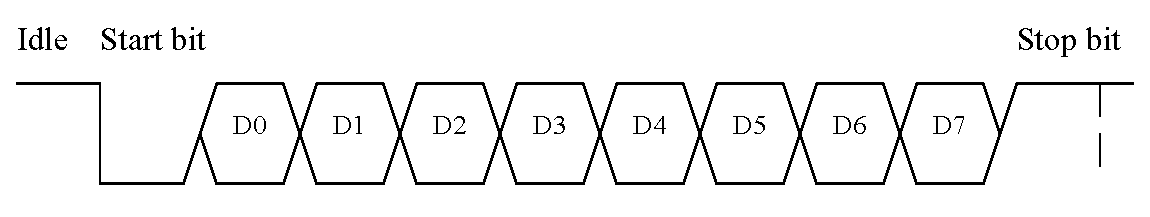
\includegraphics[scale=0.5]{images/rs232}
  \caption{RS-232 data transmission scheme for 8 data bits (D0-D7)}
  \label{fig:rs232}
\end{figure}

Our implementation will focus on just one possibility for all these values,
in the common shorthand, we use `115200/8-N-1', meaning that
the baud is 115,200 bits per second, there are 8 data bits, no parity bits
and 1 stop bit. The timing digram for this implementation can be seen in Figure~\ref{fig:rs232}.
While RS-232 can utilise extra handshaking signals for flow control, such as software
flow control with `XOFF' and `XON' signals,
these are not required and so are not implemented.
However, without
any flow control the timing of the transmission is of even greater importance
to the protocol. With a baud chosen of 115,200 bits per second we need to generate
a clock pulse with a period of $\dfrac{1}{115200}$ seconds, or approximately
$868 \mu s$. A master clock of 50MHz is provided by the development board.
Using this as a basis for keeping syncronised to the baud rate necessitates the
implementation of a clock divider which implements a counter
that counts 434 rising edges of the master clock ($\dfrac{50MHz}{115200}$)
before reseting. There is also a counter for tracking progress through the 8
separate data bits processed.

The design of a \gls{uart} is split into two distinct halves; the transmitter
and the receiver. Each operates somewhat independently.
Each half requires a separate set of two of counters; \emph{frequency} and \emph{bit},
counting down to 0 before resetting back to 434 or 8 respectively:
\begin{itemize}
  \item \inlinecode{FRQ\_CNT\_RX} - Baud Counter for Receiver
  \item \inlinecode{FRQ\_CNT\_TX} - Baud Counter for Transmitter
  \item \inlinecode{BIT\_CNT\_RX} - Bit Counter for Receiver
  \item \inlinecode{BIT\_CNT\_TX} - Bit Counter for Transmitter
\end{itemize}

\subsubsection{Receiver}

The receiver is required to convert serial input into an 8-bit parallel output.
Hence a \gls{sipo} shift register is used in this half of the \gls{uart}.
Transmission is handled through a case analysis, triggered every rising edge of
the master clock which sets output depending on its two counters:
\begin{description}
\item[If \inlinecode{BIT\_CNT\_RX = 0 AND FRQ\_CNT\_RX = 0}] \hfill \\
  In normal circumstances this is the idle state. However, if the receiving signal is
  low it means that a start bit has been encountered and the module starts receiving
  a byte by resetting both counters.
\item[If \inlinecode{BIT\_CNT\_RX < 8 AND BIT\_CNT\_RX < 0}] \hfill \\
  Writing the current bit of the bit of the \gls{sipo} it indexes, noting that the
  RS-232 protocol is little-endian. If this is the last bit, then set the strobe (STR)
  and decrement the bit counter for the final time this cycle.
\item[Default Case] \hfill \\
  Decrement the frequency counter.
\end{description}

\subsubsection{Transmitter}

The transmitter is required to convert an 8-bit binary input into a serial output.
Hence, a \gls{piso} shift register is used in this half of the \gls{uart}.
Transmission is also handled through a case analysis triggered every rising edge of
the master clock as follows:
\begin{description}
\item[If Transmission Strobe (STT) is high] \hfill \\
  Set the RS-232 output signal low to indicate the start bit and reset counters.
\item[If \inlinecode{FRQ\_CNT\_TX = 0 AND BIT\_CNT\_TX > 0}] \hfill \\
  Set the output to the bit of \gls{piso} register indexed by the bit counter,
  decrement the bit counter and reset the frequency counter. Again, note that the
  RS-232 protocol is little-endian.
\item[If \inlinecode{FRQ\_CNT\_TX=0 AND BIT\_CNT\_TX=0}] \hfill \\
  Last data bit was previously sent, so set the RS-232 output signal to high
  to indicate the stop bit, with both counters zeroed, the idle state is entered.
\item[Default Case] \hfill \\
  Decrement the frequency counter.
\end{description}

\subsection{SRAM-PUF Implementation}

With the two components (\gls{sram} wrapper and \gls{uart} module) created,
integration of control signals becomes a simple matter of connecting the two strobe
signals (STR and STT) together so that they interact appropriately. Then the 8-bit
data lines between the two were joined (with a separate output to drive the LEDs for
debugging purposes). The \gls{vhdl} code implementing the SRAM-PUF can be found in
\autoref{app:srampuf}.

\section{Fuzzy Extractor in MATLAB}

\subsection{Introduction}

The fuzzy extractor has two processes, the generation process and the
reproduction process.
The generation process is only used for initial set-up, whereby the expected
responses for all possible challenges are generated and securely stored.
This process is likely to happen during manufacturing of the device at the
factory.
The reproduction process on the other hand, is the commonly employed procedure
whereby for a given challenge a response is generated that can be tested against
the initial response from the generation process.
These are implemented differently because in the generation process, both a
response and helper data must be generated. In the reproduction process, helper
data is consumed and only a response is generated.

The core difference between the processes occurs in the secure sketch process.
In generation, a ‘sketch’ is made and the required response is recorded. This
‘sketch’ results in helper data to be used in the reproduction procedure and is
stored in such a way that it can be sent with all challenges used in the
challenge-response protocol. In reproduction, a ‘recovery’ is performed,
whereby the previously generated helper data and the noisy input from the \gls{puf}
are processed to produce an input for the randomness extractor.

\subsection{Helper Data}
The helper data is required both to allow for differences in the raw responses
of the \gls{puf} and to keep the data cryptographically secure. One is associated
with the secure sketch components (let us call this `$s$'). The other is associated
with the randomness extractor (let us call this ‘`$x$'’).
As the design is both quite complex and nuanced, it is difficult to explain at
once. However, much of the overarching
functionality of the fuzzy extractor can be explained following the path of the
helper data as shown diagrammatically in figure~\ref{fig:generation}
and figure~\ref{fig:reproduction}
 before exploring the major components in detail.

\begin{figure}
  \centering
  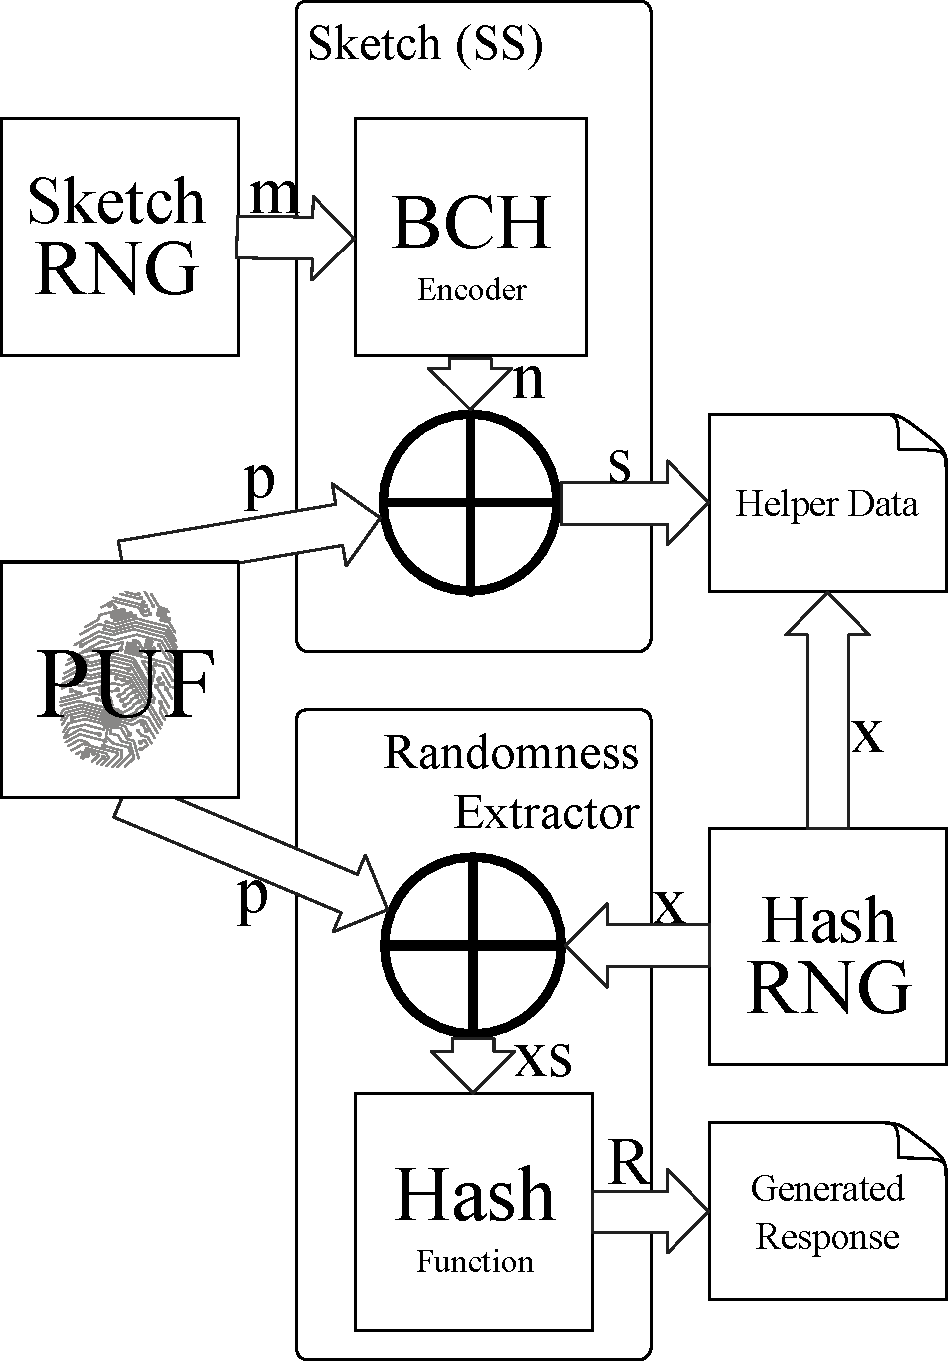
\includegraphics[scale=0.7]{images/generation}
  \caption{Fuzzy Extractor Generation Process}
  \label{fig:generation}
\end{figure}

\begin{figure}
  \centering
  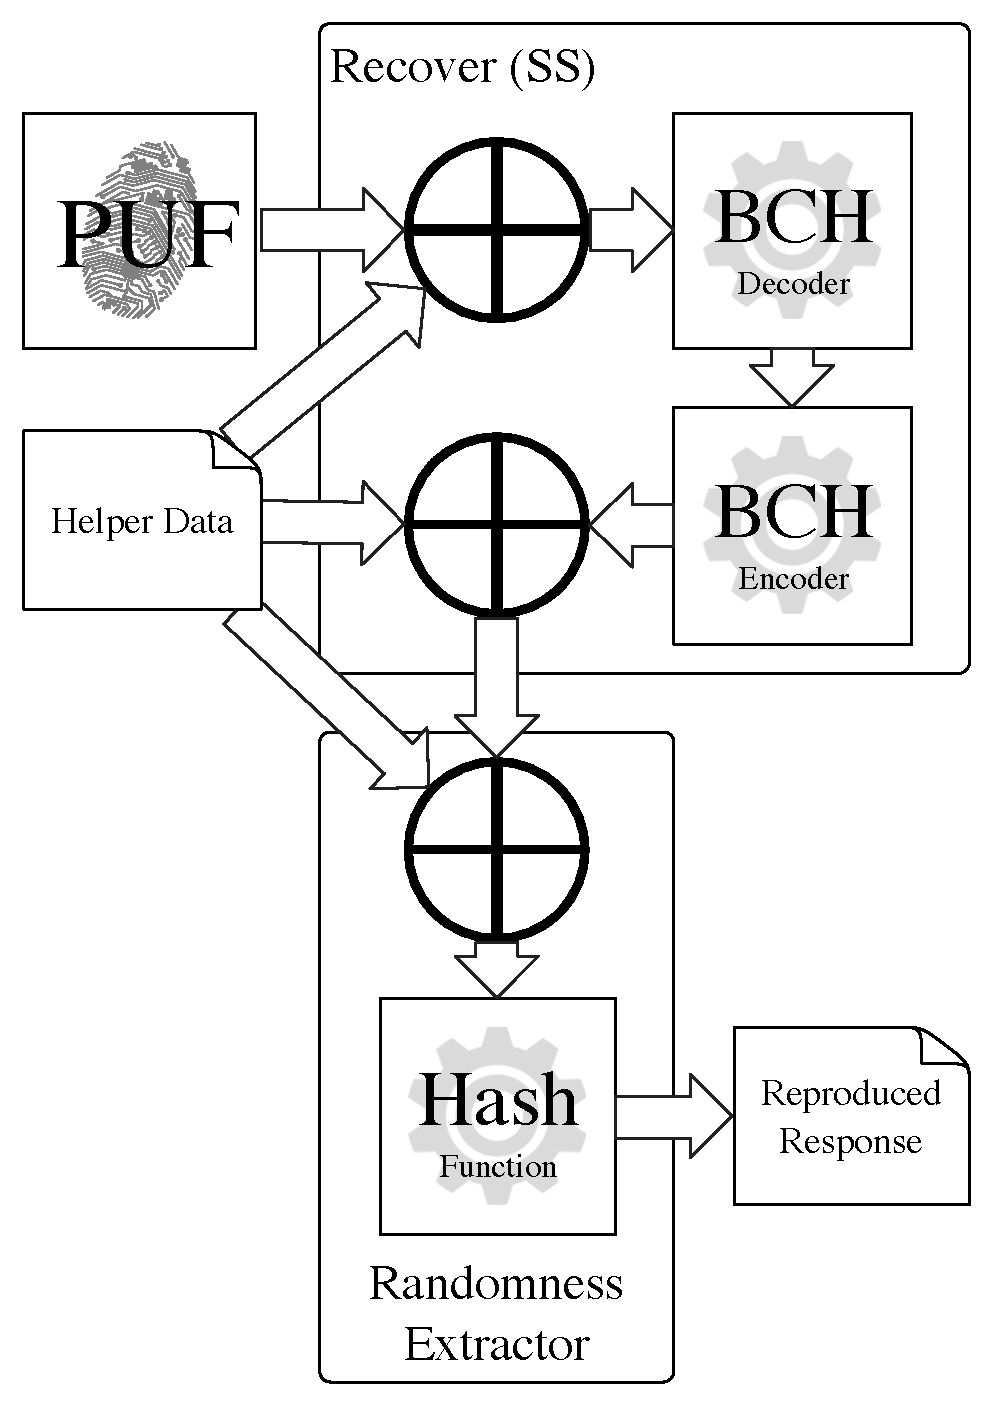
\includegraphics[scale=0.7]{images/reproduction}
  \caption{Fuzzy Extractor Reproduction Process}
  \label{fig:reproduction}
\end{figure}

In generation the secure sketch outputs redundant data $n$ which is the
same length as the raw data from the puf $p$. These are combined with the
XOR operator and the result is the helper data $s$ ($p \oplus n = s$).
In reproduction $s$ is used twice,
once when it is combined with new (fuzzy) \gls{puf} data $p'$ (note the dash)
using an XOR operation.
Due to the information preserving, cyclical nature of the disjunctive
operator (XOR) the result is therefore a potentially fuzzy version of the encoded message
($s \oplus p' = n'$).
It is XORed again to reproduce the original \gls{puf}
data by using the XOR operation on the encoded message, but after it has been
`cleaned up' (ie. $s \oplus n'' = p'' \approx p$).
Thus $s$ is, in effect, the secure \emph{sketch} itself, encrypted by a key analogous
to a \gls{otp} made from the \gls{puf} data.

The other helper data is used in the randomness extractor and is used to
generate a Privacy Amplified response. In generation, random data is captured
from a \gls{trng} and stored as helper data $x$. Simultaneously, input
from the \gls{puf} is combined with it through an XOR
operator (let us call the output of this operation $xs$, so $p \oplus x = xs$)
which is applied as the input a
cryptographic hash function which outputs the original response.

In reproduction, the same input to the randomness extractor is used to output
the same response.
If it is assumed for now that the secure sketch recovery component provides the
original \gls{puf} data, by XORing it with $x$ again we should create the same input to the
cryptographic hash function as in the generation process, thus the same response
will be generated. This means that $x$ is analogous to a \gls{otp} used to
encrypt in original \gls{puf} data.

\subsection{Secure Sketching}

More accurately, the ‘\emph{sketch}’ used in the generation process takes in two
inputs; the first is the raw data
from the \gls{puf} that is known to be noisy and the second is random data generated
by the first of two independent \glspl{trng} (we shall name
this the ‘'Sketch RNG'’ in future as it is used by the Secure Sketch part of the
fuzzy extractor). The random data, which we shall call ‘`$m’$' for `message', is passed into a
BCH-encoder sub-component that therefore generates a redundant encoding of that
random data which we shall call `$n’$' which can later be error-corrected during the
‘recovery’ stage. The length of the message must always be less than the
encoding. The smaller it is, the more errors that can be corrected.

This encoded message is then XORed with the \gls{puf} data ($p$) to create the first of
the two pieces of helper data $s$. It is therefore important that the output of the
BCH encoder is identical in size to the raw input data from the \gls{puf}.
The other part of the helper data is a second random data block generated by the
second of the \glspl{trng} (we shall call this the `‘Hash RNG'’
in future as it is used in the \emph{privacy amplification} part of the fuzzy extractor
which primarily involves hashing). Again, $‘x$’ must be the same size as $p$.
Ultimately, this process securely generates helper data from the
raw \gls{puf} (and therefore noisy) data by which the second process, the
‘recovery’, will be able to reproduce as output the same \gls{puf} data as that
encountered in the initial generation procedure, even if the \gls{puf} outputs
slightly different data.

The \emph{recovery}’ also takes in two inputs. The first is raw input from the \gls{puf} ($p'$)
which, to reiterate, is likely to be different from the first time (hence the dash).
The second is the ‘helper data $s$. By XORing them together we produce a potentially
noisy version of the original output of the BCH encoder ($n$) and then using that
as the input to a BCH-Decoder, we can use the properties of forward error
correction to duplicate the original message created by the sketch \gls{rng} used in the
generation procedure.
If we then pass that into a BCH-encoder, we will get exactly the same data that
was originally combined with the \gls{puf} output.
If we then XOR this with the same helper data $s$ a second time, we reproduce the
original output of the \gls{puf}.

Thus, we have potentially recovered, error-free, the data used in generating the
response. This means that the fuzzy extractor works as desired, and slight changes
in raw \gls{puf} data can be mitigated. However, if there are more errors than can be
corrected by the BCH decoder used, the data will not be recovered correctly.
This has two important consequences. Firstly, the BCH encoder should be capable
of correcting enough errors such that all but the most extreme degradation of
the \gls{puf} can be accounted for. Secondly, it can be seen that without the
functionality of the randomness extractor, i.e. if $xs$ was taken as the response
 of the fuzzy extractor instead of passing it through a hash function, a
security risk occurs. This is due to the BCH-encoding process `correcting' errors in the response.
This means that an attacker can use repeated guessing of a response to a
particular challenge in what is known as a `bit-flipping attack'
 and each time it will be capable of learning some parts
of the original response through pattern analysis.

\subsection{Randomness Extracting}

When the recreated \gls{puf} data `$p$' is XORed with the helper data `$‘x'$'
(which is the original output of the Hash-RNG) this should
be expected to match the message that was applied to the SHA-256 cryptographic
hash function in the original generation procedure.
The nature of a hash function is such that, given the same message, and the
exact same initial parameters, the function
\emph{must} produce the same digest.
Thus the response in the reproduction procedure will be the same as in the
generation procedure even with slight differences in raw \gls{puf} data.

However, the purpose of the hash function is to throughly scramble the data in
such a way that the input cannot be deduced from the output alone. This means
that even a slight change (one bit flipped) in the input should result in a
radically different output. This is commonly known as the \emph{avalanche effect}\cite{feistel1973cryptography}.

Through this, the \gls{puf} data is hidden and never revealed in plain-text.
It is cryptographically assured and thus authentication of the \gls{puf} is
performed securely. A incremental `bit-flipping attack' is prevented as no
patterns can be gleaned from the response.
Even though helper data ($s$ and $x$) is available to the attacker, this will not give away
the \gls{puf} key, as we can trust the mathematically rigorous cryptographic security
of the SHA-256 hash function to obfuscate the response/digest output such that
the original \gls{puf} cannot be retrieved from it, as it is the `key' used to
`encrypt' the sketch output `$n$' keeping it secret prevents any attack.

\subsection{Bus Width Considerations}
The response produced by both fuzzy extractor processes is fixed by the nature of
the SHA-256 hash function, which has a 256-bit output.
Furthermore, assuming that the output of the \gls{puf} is a block of data of length
‘$w$’ and the SHA-256 hash function and BCH encoder are used the length $‘w’$ is
somewhat limited.
For purposes of cryptographic strength (to be looked into further in \autoref{sec:hash}
on Cryptographic Hashing) the length of the encoded message $n$’ should be one
less than an integer power of 2.
Since the \gls{puf} data $p$ is bit-wise combined with $n$ it should be the
same length. However, due to the 16-word length of the data it would be sensible
to use an exact power of 2 output and simply drop the \gls{msb}.

It also
simplifies the implementation to limit the input of the SHA-256 component to a
single 512-bit block. By avoiding the development of complex functionality,
necessitating extra memory requirements and adding greater potential latency a multi-block
implementation would involve, the design is simplified while ensuring that
little cryptographic strength is lost.
This means
that the upper limit for \gls{puf} data is actually no greater than 440 bits.
This is because the SHA-256 input message is appended with a stop bit
and 64 bit length field and as the \gls{puf} output comes in 16-bit words,
the largest multiple of 16 that will fit into $512 - 65$ bits is 440.
This therefore limits the reasonable choices
for the size of \gls{puf} data to be either 64, 128 or 256 bits in length.

Due to the contraction entailed in matching the raw \gls{puf} input to the
code length of the BCH encoder
the $s$ and $x$ helper data will both also be initially created one bit smaller
than the corresponding \gls{puf} data length (ie. 62, 127 or 255 bits).
However a `0' MSB
is added to conform the data to conventional power of 2 bus widths, hence
they will also be the same size. In the main implementation of the system, a data
length of 128 was chosen, but the modular nature of the design was used to
allow for experimentation with the other two options.
The exact size of the sketch-RNG output, which corresponds to the length of the
plain, uncoded message `$m$' is all that is now left to define. The nature
of BCH encoding limits the efficient choices to a small list (see the
correctable errors tables - \autoref{tab:bch63},
\autoref{tab:bch127} and \autoref{tab:bch255}).
Even limited to a finite list, there is no
obvious `correct' value for this and necessarily involves a compromise.
A smaller
message allows more errors to be corrected, conversely, a larger one provides more entropy and
adds greater security to the system. The main implementation demonstrated uses
a message length of 64 bits, but again this is set by a parameter that can easily be
changed in the code.

\subsection{Components Required by the Fuzzy Extractor}

To implement our complete fuzzy extractor in \matlab the following sub-components
must be created, correctly tested and connected together correctly:

\begin{description}
\item[BCH Encoder] \hfill \\
Used once in generation and once in the reproduction procedure.
\item[BCH Decoder] \hfill \\
Used only once in the reproduction procedure.
\item[SHA-256 Hash Function] \hfill \\
Used once in the generation and once in the reproduction procedure.
\item[True Random Number Generator] \hfill \\
Used twice, both times in the generation procedure
(\emph{Hash-RNG \& Sketch-RNG}).
\item[Bitwise XOR] \hfill \\
Used twice in the generation procedure and
three times in the reproduction procedure.
\end{description}

The code implementing the fuzzy extractor can be found in \autoref{app:fuzzy}.

\section{BCH Encoder and Decoder}

\subsection{Introduction and Theory}

Forward error correction codes are methods for the transmission and reception
of data such that noise is mitigated and the original data sent is transferred
without error.
All implementations require an encoder which adds redundancy to the message to
be transmitted and a decoder which can use that redundancy to recover the
original message even if the transmitted data is disturbed and unwanted
alterations are introduced.
It is important to contrive a system that is both efficient in the resources it
uses (both time and area it requires) and is accurate and powerful enough to
correct the peak amount of errors expected due to noise.

Error correcting codes can be classified into a hierarchical tree of types.
One of the broadest branches of that tree are linear block codes,
of which BCH is one form.
Linear codes are a class of error correction codes in which addition is
‘closed’ this means the code is cyclic in the same sense as modular arithmetic.
BCH codes are in the sub-class of linear codes called block codes.
These function opon the original message one block at a time. An alternate scheme
is to use convolution codes such as the Viterbi\cite{viterbi1967error},
which function continuously on
streams of data. However, for the purposes of the fuzzy extractor such codes simply
adds extra complexity since the responses are fixed in size which suits block
encoding.
Recent research has been directed to even more efficient codes (such as Turbo
or Raptor code) these approach the theoretical limits of coding theory
(Shannon limit) but are similarly out of the scope of this project.

BCH codes are of a specific sub-class of cyclic linear block codes – those of
which utilise a binary encoding, this is also the case for the simpler Hamming
codes, but is unlike other block codes such as Reed-Solomon or Reed-Muller
which use a larger symbol set.
For brevity, we adopt the convention that the encoder takes a block of symbols
length ‘m’ and that it translates into a larger block of length ‘n’ by adding
redundancy.
In any encoding system the symbols used in the message block are taken from an
alphabet ‘A’ which has ‘q’ symbols (therefore there are $q^{m}$ and $q^{n}$
possible message and digest block sequences).
Therefore we can define any block code in the form: $a (n, m)$-block code called
$‘C’$ over the alphabet $‘A’$ with $‘q’$ symbols. An encoder for the block code
$‘C’$ (let us call it $‘E’$) is a bijective mapping such that there is an exact
one-to-one correspondence between the original message ($‘M’$) and the encoded
message ($‘T’$).

The simplest block codes are the Hamming codes.
These are capable of correcting only one random error, and are therefore not
useful in this project.
The BCH code is more sophisticated and can be seen as a generalisation of the
Hamming codes for multiple-error correction.
Mathematically BCH codes operate over finite fields (in simple terms this as the
same as ‘modular arithmetic’) these can also be called Galois fields after their
discoverer the 19th century French mathematician \'{E}variste Galois.
The order of the field is the number of elements it contains, and for BCH codes
the size of the Galois field is two or $GF(2)$. The key property of finite
fields is that they allow for the basic operations of addition, subtraction,
multiplication and division to be used while holding to six conditions:

\begin{description}
\item[Closure] \hfill \\
For all operations on two operands that are elements of the finite field F the
result is also an element of the field (i.e.  $c=a+b$ where $a,b,c \in F$).
\item[Associative] \hfill \\
Two like operations applied in either order will cause the same result
(i.e.  $a+(b+c)=(a+b)+c$ )
\item[Identity] \hfill \\
There exists identity elements such that for all operations the result is the
same as the other elements (i.e. $0 + a = a$ where ‘0’ is the identity for addition
and $1 \times b = b$ where ‘1’ is the identity for multiplication)
\item[Commutative] \hfill \\
Where order of operands does no’t change the result (i.e. $a + b = b + a$ )
\item[Inverse] \hfill \\
There is an ‘inverse’ element for every element in the field that the result is
the operator’s identity element. (i.e. $a + b = 0$, where b is the additive
inverse, and  $a \times c = 1$, where c is the multiplicative inverse)
\end{description}

It has been shown that the set of integers {$0, 1,..,p-1$} where p is a prime
number and where all operations are performed modulo ‘p’ are valid finite fields
of order ‘p’.
As 2 is the first prime number the Galois field used by BCH is the simplest
finite field, it is also much easier to map to the digital domain of binary
numbers.
Larger fields can be used in error correcting codes. These can often result in
greater encoding efficiency, but are harder to implement and for our purposes
the efficiency increase is of rather limited usefulness due to the small size
of the responses expected.

\subsection{Implementation}

As previously stated, the implementation of a BCH encoder in \gls{fpga}
was not attempted, neither was the implementation of the \matlab code necessary
to perform the calculations.
Instead, the BCH implementation in the \matlab Communications Systems Toolbox was employed.
Adequate understanding of the mathematical principals of the BCH code was
required for informed usage of the BCH functions and tools provided in the \matlab environment.
It was important to understand the errors that could be corrected by the different
parameters under which a BCH encoded message could be generated.
Efficient BCH code lengths are somewhat set by the properties of the cyclic
codes used. Efficient implementation entails BCH code lengths ('$n$') that
have the form $2^{m}-1$,
where m is an integer i.e.

$ \left\{ n | \exists m \in \mathbb{N} \wedge n = 2^{m} -1  \right\} $.

Further \matlab computations limitations limit the value of m to between 3 and 16.

Thus, considering anything below 16-bits is wasteful as that is the minimum
memory data retrieved and anything extremely large would be expensive in terms
of system resources. Hence, 31, 63, 127, 255, 511 and 1023 are the
choices available for efficient code length. as the corresponding outputs
from the \gls{puf} will necessarily be multiples of 16, the \gls{msb} of the \gls{puf}
was dropped for it to conform to the sketch system.
For the purposes of \gls{puf} implementation a width of 127 for the input bus was chosen.
Testing was also carried out in simulation of other widths for comparison.

The size of the message encoded by BCH has direct effects on the number
of errors that can be corrected in the decoder. The \matlab function
\inlinecode{bchnumerr(N)} can be used to calculate these values;
where \inlinecode{N} is the code length. The results of running the
function for code lengths of 63, 127 and 255 are shown in \autoref{tab:bch63},
\autoref{tab:bch127} and \autoref{tab:bch255}. Note that $n$ is the code
length, $m$ is the message length and $d$ is the number of errors that can be
corrected. Using these tables it was
decided that for project demonstration purposes it would be best to use a
message size of 64 bits which is approximately half the size of the code length.
The reasons for this were three-fold: Firstly it covered for the possibility of
one complete byte of memory data being corrupted in the RS-232 communication
channel (seen as a possibility given the lack of parity checking).
Secondly, it would ensure adequate entropy, as with a small message size a
brute-force attack could be mounted. Whereas with $2^{64}$ possible messages it
would be infeasible. Thirdly, it was also admittedly, simply an aesthetic choice of a power of 2.
This last point demonstrates that further investigation into the consequences
and inherit compromises made in any particular message length choice would be of
interest.

\begin{table}
\begin{tabular}{lll}
\hline
 n  &   m &   d \\ \hline
 63 &  57 &   1 \\
 63 &  51 &   2 \\
 63 &  45 &   3 \\
 63 &  39 &   4 \\
 63 &  36 &   5 \\
 63 &  30 &   6 \\
 63 &  24 &   7 \\
 63 &  18 &  10 \\
 63 &  16 &  11 \\
 63 &  10 &  13 \\
 63 &   7 &  15
\end{tabular}
\caption{Number of correctable errors for BCH code length of 63}
\label{tab:bch63}
\end{table}

\begin{table}
\begin{tabular}{lll}
\hline
n   &   m &   d \\ \hline
127 & 110 &   1 \\
127 & 113 &   2 \\
127 & 106 &   3 \\
127 & 120 &   1 \\
127 & 113 &   2 \\
127 & 106 &   3 \\
127 &  99 &   4 \\
127 &  92 &   5 \\
127 &  85 &   6 \\
127 &  78 &   7 \\
127 &  71 &   9 \\
127 &  64 &  10 \\
127 &  57 &  11 \\
127 &  50 &  13 \\
127 &  43 &  14 \\
127 &  36 &  15 \\
127 &  29 &  21 \\
127 &  22 &  23 \\
127 &  15 &  27 \\
127 &   8 &  31
\end{tabular}
\caption{Number of correctable errors for BCH code length of 127}
\label{tab:bch127}
\end{table}
\begin{table}
\begin{tabular}{lll}
\hline
n   &   m &   d \\ \hline
255 & 247 &   1 \\
255 & 239 &   2 \\
255 & 231 &   3 \\
255 & 223 &   4 \\
255 & 215 &   5 \\
255 & 207 &   6 \\
255 & 199 &   7 \\
255 & 191 &   8 \\
255 & 187 &   9 \\
255 & 179 &  10 \\
255 & 171 &  11 \\
255 & 163 &  12 \\
255 & 155 &  13 \\
255 & 147 &  14 \\
255 & 139 &  15 \\
255 & 131 &  18 \\
255 & 123 &  19 \\
255 & 115 &  21 \\
255 & 107 &  22 \\
255 &  99 &  23 \\
255 &  91 &  25 \\
255 &  87 &  26 \\
255 &  79 &  27 \\
255 &  71 &  29 \\
255 &  63 &  30 \\
255 &  55 &  31 \\
255 &  47 &  42 \\
255 &  45 &  43 \\
255 &  37 &  45 \\
255 &  29 &  47 \\
255 &  21 &  55 \\
255 &  13 &  59 \\
255 &   9 &  63 \\
\end{tabular}
\caption{Number of correctable errors for BCH code length of 255}
\label{tab:bch255}
\end{table}


\section{SHA-256 Algorithm Implementation on FPGA}
\label{sec:hash}

\subsection{Theory of Cryptographic Hash Functions}

Hash Functions in simple terms, are a mapping from an input data called the
\emph{message} to output data called the message \emph{digest}.
Mathematically, this mapping is \emph{surjective}, i.e. it guarantees
that \textbf{all} possible inputs map to some valued output.
However it is not a \emph{bijection} because it is not \emph{injective}.
Therefore, in a hash, there may be \emph{more than one} input that maps to
the same output.
This possibility means it is conceivable for a hash \emph{collision} to occur,
although this can be made extremely unlikely in practice through the use of
universal hashing algorithms.

Cryptographic hash functions are a subset of all hash functions.
Their defining attribute is that the function must be as \textbf{one-way} as
possible.–
It should be, if not theoretically then practically impossible to perform the
inverse function of creating a valid message given some digest.
The degree of difficulty for an adversary breaking a given system will increase
in some complexity order related to the digest length.
Making this order as large as possible is key to a strong hash function.
For the SHA-2 hash family, which is to be implemented in the project, a brute force
attack can only be done in exponential time ($O(c^{n}), c > 1)$).
Hence, by using a large enough digest size (and due to compounding nature of
exponential growth the size in bits need not be very large at all) a
\emph{pre-image} attack (i.e. one try to find a message for a given hash)
will be prevented.
This only holds true as long as serious security flaws in the SHA-2 algorithm
allowing some shortcut are not found in the near future; which would seem
somewhat unlikely; excluding advances in quantum computing.

Another form of attack that needs consideration is the
\emph{‘second pre-image} attack.,
whereby a second message is found with the same digest as a set first message.
Again this form of attack is secured against by SHA-256 well.
The final style of attack considered is that of a \emph{collision} attack,
whereby two messages (neither set) are found which result in a collision.
This is the easiest attack to mount, and generally any attacks found in the
literature are of this type. So far, a collision attack of the SHA-2
family has not been found, although non-standard reduced versions of the
SHA-2 family and the older, related SHA-1 standard are
vulnerable\cite{sanadhya2009combinatorial}.

An explanation of the functionality of the SHA-256 hash function would be
appropriate to explain the choices made in its implementation.
Although the design (as shown in figure~\ref{fig:sha256})
seems rather convoluted, this is a product of the nature of
the function. Its purpose is to jumble the data in the message as thoroughly as
possible in the minimum amount of time and space.
Hence it uses a lot of complex logical operations in a complex sequence, but
there is no other ‘meaning’ or purpose behind the design other than that it has
been found through experimentation or mathematical analysis to ‘jumble’ well.

The SHA-2 family use six different logic functions (operating on 32 bit inputs
and outputs). These are:

\begin{itemize}
	\item $Ch(x, y, z)  = (x \wedge y) \oplus (\neg x \wedge z)$
	\item $Maj(x, y, z) = (x \wedge y) \oplus (x \wedge z) \oplus (y \wedge z)$
	\item $\Sigma_{0}(x) = ROTR^{ 2}(x) \oplus ROTR^{13}(x) \oplus ROTR^{22}(x)$
	\item $\Sigma_{1}(x) = ROTR^{ 6}(x) \oplus ROTR^{11}(x) \oplus ROTR^{25}(x)$
	\item $\sigma_{0}(x) = ROTR^{ 7}(x) \oplus ROTR^{18}(x) \oplus  SHR^{ 3}(x)$
	\item $\sigma_{1}(x) = ROTR^{17}(x) \oplus ROTR^{19}(x) \oplus  SHR^{10}(x)$
\end{itemize}

Where $ROTR^{n}$ means a \emph{rotate right} function by $n$ bits, $\oplus$ is
the exclusive or operator, $\wedge$ is the bitwise AND operator and finally,
note well that the last x in the first function is negated ($\neg$).

Note that all these functions can be synthesised on an \gls{fpga}, as should be
expected, as the SHA-2 was designed to function well in hardware.
The SHA-256 function operates on block sizes of 512-bits, and produces a
256-bit digest.
In operation, that 256-bit digest is stored in 8 32-bit buffers
($H_{0} - H_{7}$).
Also to be stored are 8 intermediate 32-bit hash registers
(note $8 \times 32 = 256$) labelled alphabetically ‘$a$’ to ‘$h$’.
Both buffer and registers are first initialised to a set of constant values
(generated from calculating the square roots of the first 8 prime numbers).
The message block is split into 16 32-bit values ($W_{0} - W_{63}$), whereby the
message gets ‘fed’ into the main part of the function one at a time in a queued
fashion, each ‘feed’ occurring during a ‘round’ of operation.
Added complexity is introduced by also feeding the front value back into
the queue using the two bottom s operations such that for the current round
‘j’:

$W_{j} \Leftarrow sigma_{1}(W_{t-2} )+ W_{t-7}  + sigma_{0}(W_{t-15}) + W_{t-16}$.

This sounds complicated, but can be implemented as a large \gls{lfsr}.
Note, there is usually a padding step, but padding is not necessary in our
implementation as we can ensure our values fit exactly the
512-bit message block required.

Normally the function is used to hash large messages that are split into
multiple blocks. In our implementation only a single block is sufficient for
security, which simplifies the implementation by removing an outer loop from the
standard algorithm.
The important step is to apply the SHA-256 compression function for 64 rounds,
in each of which updates of all the registers are made and more of the message
block is added piece by piece. The updates are as follows:

\begin{itemize}
	\item $T_{1} \leftarrow h + \Sigma_{1}(e) + Ch(e,f,g) + K_{j}  + W{t}$ (n.b.. where $K_{j}$ is one of 64 standardised 32-bit constants)

	\item $T_{2} \leftarrow \Sigma_{0}(a) + Maj(a,b,c)$
	\item $h     \leftarrow g$
	\item $g     \leftarrow f$
	\item $f     \leftarrow e$
	\item $e     \leftarrow d + T_{1}$
	\item $d     \leftarrow c$
	\item $c     \leftarrow b$
	\item $b     \leftarrow a$
	\item $a     \leftarrow T_{1} + T_{2}$
\end{itemize}

Once the registers are set, the buffers are set to a new intermediate value by
ANDing each of the 8 registers to its corresponding buffer
(i.e. $H_{0} \leftarrow a + H_{0}, H_{1} \leftarrow b + H_{1}$ etc.).
After all 64, rounds the buffer contains the hash of the message.

\begin{figure}
  \centering
  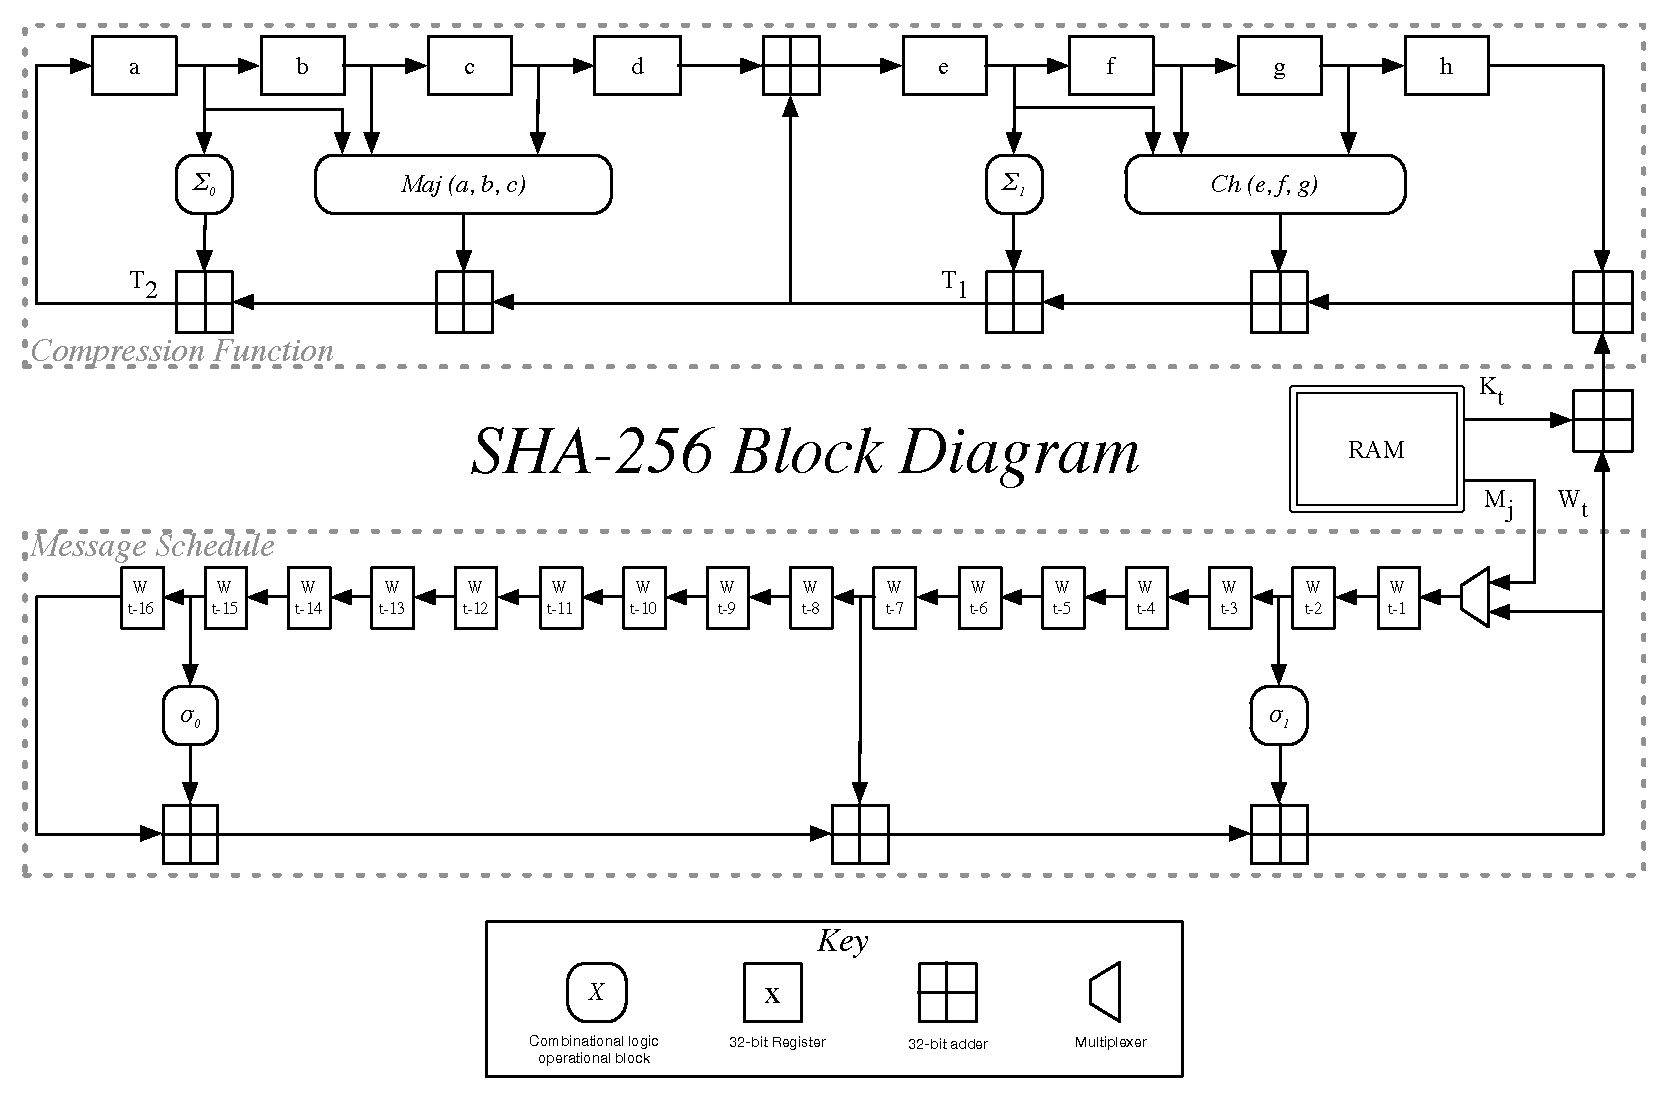
\includegraphics[angle=270, scale=0.7]{images/sha256}
  \caption{SHA-256 Block Diagram}
  \label{fig:sha256}
\end{figure}

\subsection{Implementation}

The SHA-256 function was implemented in \matlab for mostly pedagogical reasons.
There were no serious performance constraints and as such the implementation is
intentionally extremely inefficient to retain as much clarity of intent as
possible. Interestingly, there is no official library implementation of the SHA
algorithms in \matlab. The matlab code can be found in \autoref{app:sha256}.

\section{Design of New Ethernet Authentication Protocol Method}

\Gls{eap} is only a framework in which authentication methods can be incorporated.
By using the technique of following the design of a minimal pre-existing method,
while using different \gls{puf} specifics where appropriate, a new method could
be created. This approach leverages an existing framework for \gls{puf} based
authentication.

Each \gls{eap} method is indicated through a code in the \gls{eap} packet.
A new method would require a new method code.
The official types are maintained by \gls{iana}\cite{iana2014eap}.
At the time of writing the official list contains 57 reserved codes, out of the
possible 256, meaning there is room for more methods.
While actually registering a new method is out of the scope of this project, the
demonstration uses the unassigned value 192 for the new method type that is
designated `EAP-PUF'.
\footnote{Usefully, 192 is also unassigned as a RADIUS Attribute Value Pair}.
For expediency, it was determined to develop a full working \emph{simulation}
of sequence of Ethernet packets required in the `EAP-PUF' authentication procedure.
This is to avoid practical implementation difficulties while at a prototype
stage and gain an overview of the technologies and overarching design decisions
required.

The design of a complete authentication procedure intertwines two broad areas;
that of protocol packet sequencing and that of packet contents specification.

\subsection{The EAP-PUF Protocol Sequence}

Figure~\ref{fig:sequence} most clearly shows a complete authentication sequence.
As can be seen this involves three entities:

\begin{itemize}
\item The Supplicant - A device containing a \gls{puf} for verification.
\item The Authenticator - A device which represents the point of connection for nodes on the network, most likely a network switch.
\item The Authentication Server - A server that can issue and verify EAP-PUF \glspl{crp}
\end{itemize}

In a typical sequence for a basic \gls{eap} method (such as EAP-MD5, which was
most often referenced in the design of EAP-PUF) the authenticator acts a middle
man or translator in a handshake exchange between the authentication server
and the supplicant.
This two step approach is used because the authentication server is likely communicating with the
authenticator using a high layer protocol. A typically used protocol is
\gls{radius}, which happens to run in the application layer. As an intended
supplicant for \gls{puf} authentication is a low-power embedded device it may
have insufficient resources to communicate with a \gls{radius} server directly.
\Gls{eap}, being a versatile authentication framework can be transported via
any layer protocol, in this case it can be encapsulated in Ethernet between the
supplicant and authenticator using the \gls{eapol} protocol, then translated by
the authenticator into a \gls{radius} packet and visa-versa.

The process of authentication can be initiated by the authenticator
sending a EAP-Request Identity packet, but typically this can be ignored and the
supplicant can, in any case, preempt this by simply sending a \gls{eapol} Start packet.
This packet has an empty body without any \gls{eap} data. By sending this packet
the supplicant confirms that it can use the \gls{eap} protocol for authentication.

Before Authentication using the EAP-PUF the supplicant needs to
provide its claimed identity so that the appropriate authentication method can be
used, with the appropriate \gls{crp} for that identity selected.
This identity retrieval step generally involves the use of
a separate \gls{eap} method (type 1) used solely for the communication of identity. Although
in advanced methods \emph{identity protection} is promoted by bypassing this method
and using custom versions instead.
First, upon receipt of the start packet, the authenticator generates a new
identity byte for this authentication exchange to allow it to keep track of multiple
simultaneous authentication sessions and sends the identity request packet.
The supplicant then replies with its identity. These are both full \gls{eap}
packets. It is interesting to note that the authentication server is not
required up to this point. The specifics of the identity protocol body are
authentication method specific, but it is recommended in the relevant \gls{rfc}
to piggy-back a method request in the identity response packet.

When the Authenticator receives the identity response it needs to initiate \gls{radius}
communication with the authentication server with a Access-Request packet, this
includes the \gls{mac} address of the supplicant and a EAP-PUF method request. How this
is formatted in \gls{radius} is out of scope of this project, but the authentication
server is expected to respond with an Access-Challenge packet containing an
appropriate Challenge for the identity of the supplicant which is forwarded by
the Authenticator in an EAP-PUF Request packet. This needs to contain the
challenge data and the helper data. At this
point the reproduction process can be initiated on the device, as explained in
the preceding parts of this chapter.

Once a response has been reproduced, the supplicant replies to the request with
it EAP-PUF Response Packet containing just the 256-bit digest. It should be noted
that the Ethernet packet specification requires a minimum packet size of 512 bits.
Including the headers both the EAP-PUF request and response packets are smaller
than this, and hence padding is required to be added to the packet.

The authenticator translates and forwards the response to the authentication server
where validation occurs. This is a simple matter of comparing the received bit
sequence with that generated in the factory and stored in the database. Only if
the response is an exact match is an Access-Accept packet sent back to the
authenticator. At this point the supplicant is considered authentic by the
authenticator and full network access is granted. The authenticator also sends
a \gls{eap} Success packet (no other data contained) informing the supplicant of its
new status.

If the response is invalid a \gls{radius} Access-Reject message is sent instead,
the authenticator can act upon this in anyway it seems fit, but usually will in
turn send a \gls{eap} Failure packet (again no other data contained). Often
the supplicant will then request authentication by another method.

A successfully authenticated device can then send a EAPoL-Logoff packet when it
no longer requires network access. It should be noted that this exposes a
vulnerability of \gls{eap} protocol as this packet is sent in plain-text and is easy for
an attacker to spoof, thereby the attacker can implement a \gls{dos} attack by
continually issuing a EAPoL-Logoff packet for any \gls{mac} addresses it discovers
using \gls{eap} through packet sniffing.

To review, a supplicant using EAP-PUF to authenticate needs to be able to
interpret four receivable Ethernet packet types, and generate three types to
transmit as a functional minimum, these packet are summarised as follows:

\begin{itemize}
\item Received Packets
  \begin{itemize}
    \item EAP Identity Request
    \item EAP EAP-PUF Request
    \item EAP Success
    \item EAP Failure
  \end{itemize}
\item Transmitted Packets
  \begin{itemize}
    \item EAPoL Start
    \item EAPol Logoff
    \item EAP Identity Response
    \item EAP EAP-PUF Response
  \end{itemize}
\end{itemize}

\begin{figure}
  \centering
  \includegraphics[scale=0.5]{images/sequence}
  \caption{EAP-PUF authorization sequence diagram}
  \label{fig:sequence}
\end{figure}

The structure of these packets are explained in the next subsection.

\subsection{Ethernet Packet Contents}

The formating of the Ethernet packets used in EAP-PUF requires three levels of
encapsulation:

\begin{itemize}
\item The Ethernet packet contains a \gls{eapol} packet
\item The \gls{eapol} packet contains a \gls{eap} packet
\item The \gls{eap} packet contains a EAP-PUF body
\end{itemize}

This nesting can be clearly seen in \autoref{fig:ethernet}, which also shows all
of the heading fields that are required. The implementation of the EAP-PUF
protocol requires the supplicant to be able to interpret all these fields in
packets received from the authenticator and
generate the appropriate fields in its responses.

\begin{figure}
  \centering
  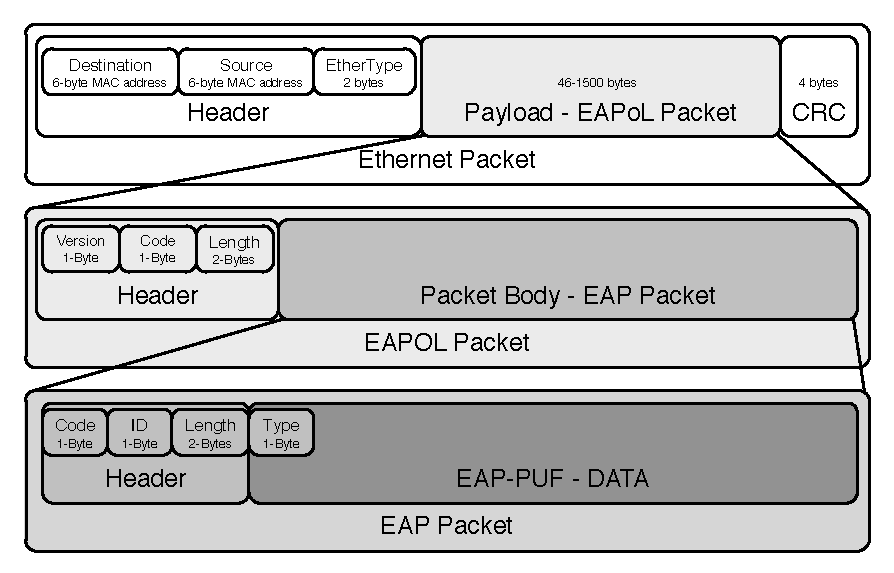
\includegraphics[scale=0.9]{images/ethernet}
  \caption{EAP-PUF encapsulated in an Ethernet Packet}
  \label{fig:ethernet}
\end{figure}

\subsubsection{Ethernet Header and FCS}

Ethernet packets consist of a header, body and a 32 bit \gls{fcs}. The header
contains the destination and source as 6-byte \gls{mac} addresses which
should be globally unique identifiers. In the \gls{eapol} protocol an additional
address is used in \gls{eapol} start packets which is a reserved group-multicast
address assigned specifically to \glspl{pae} (which are synonymous with \gls{eap}
Authenticator devices). This is used by the supplicant at the start, as it does
not know the \gls{mac} address of authenticator of the network at first. The Address
is \inlinecode{0x0180C2000003}. The Ethertype is 2 byte field which for \gls{eap}
is always set to \inlinecode{0x888E}.

After this comes the encapsulated \gls{eapol} payload followed by the \gls{fcs}.
The \gls{fcs} is used to detect communication errors through the use of a \gls{crc}. The
header and body of an Ethernet packet are checked before sending and the \gls{crc}
is computed and appended to the packet. The receiver also computes the gls{crc}
when it receives a packet and if it is different to the one attached discards that packet
without any further action being taken.

\subsubsection{EAPoL Packet Header}

\Gls{eapol} is, for the most part, a wrapper around \gls{eap} packets when sent
via Ethernet. It does also contain functionality necessary to initiate and end \gls{eap}
authentication sessions.
Its header consists of \emph{version}, \emph{type} and \emph{length} fields.
The version field is 1 byte long and, as version 2 was standardised in 2004, it
can in all likelihood be considered a static field, always containing the value
\inlinecode{0b00000010}.

The type field represents whether the \gls{eapol} packet encapsulates a \gls{eap}
packet or not. It it does not then it is a start or stop packet (other codes exist,
but are rarely used and not considered for the purposes of this project). The
code values used can be seen in \autoref{tab:eapoltype}.

\begin{table}
\begin{tabular}{ll}
\hline
EAPoL Type & Name  \\ \hline
0000 & EAP-Packet \\
0001 & EAPOL-Start \\
0010 & EAPOL-Logoff \\
\end{tabular}
\caption{EAPoL Type Codes}
\label{tab:eapoltype}
\end{table}

The length field specifies the length in bytes of the \gls{eap} payload (it is
zero if the \gls{eapol} packet is not a `EAP-packet' type).

\subsubsection{EAP Packet Header}

The \gls{eap} packet header consists of the fields; \emph{code}, \emph{identity}
and \emph{length}.

The code field is 1 byte long and the main codes
available can be seen in \autoref{tab:eaptype}, although there are other less
used extensions which are not considered in this project.
The success and failure types contain no body content and are sent from the
authenticator to the supplicant at the end of the validation process.
The Request type is also sent from the authenticator and contains a EAP-PUF
challenge in the body.

\begin{table}
\begin{tabular}{ll}
\hline
EAP Type & Description  \\ \hline
1 & Request \\
2 & Response \\
3 & Success \\
4 & Failure \\
\end{tabular}
\caption{EAP Types}
\label{tab:eaptype}
\end{table}

The body of the \gls{eap} packet first contains a method type (which in certain
respects can be seen as part of the header). This is 1 byte in length, and is set to either
the identity type (1) in the first part of the authentication sequence or the
EAP-PUF method type (192) when using EAP-PUF. A selection of common methods are
listed in \autoref{tab:eapmethod}.

\begin{table}
\begin{tabular}{ll}
\hline
Method Value & Description  \\ \hline
  0 & Reserved \\
  1 & Identity \\
  2 & Notification \\
  3 & Legacy Nak \\
  4 & MD5-Challenge \\
  5 & One-Time Password (OTP) \\
 13 & EAP-TLS \\
 18 & GSM Subscriber Identity Modules (EAP-SIM) \\
 21 & EAP-TTLS \\
 25 & PEAP \\
 26 & MS-EAP-Authentication \\
 43 & EAP-FAST \\
192 & EAP-PUF \\
\end{tabular}
\caption{Selected EAP Method Codes}
\label{tab:eapmethod}
\end{table}

The request packet for identity contains only an additional 1 byte method type
indicating EAP-PUF should be used in the response packet. The supplicant can
indicate a desire to use another method by sending a response with a \gls{nak}
method type, but this feature is not considered in the final design.
For an actual EAP-PUF request the challenge data (16 bytes)
and helper data (32 bytes) make up the rest of the body.
This data is extracted by the supplicant and passed into the SRAM-PUF and fuzzy
extractor to generate a response.

The identity response packet consists of a one byte method type containing the code
for EAP-PUF, as agreement to the usage of this method and the supplicants
identity which is its own \gls{mac} address (6-bytes). This is deemed sufficient
identification of the device, and is identical to the scheme used in EAP-MD5
but could easily be spoofed in practice. Further extensions to the
protocol could include extra protection from \gls{mac} address spoofing.
The actual EAP-PUF response packet contains the response data (256 bit digest)
and nothing else, again this follows the pattern used in EAP-MD5.

\subsubsection{simulation}

Only a simulation of the EAP-PUF authentication scheme was implemented, the
code can be found in \autoref{app:eappuf}.
